% Basic drawings
% https://www.sharelatex.com/blog/2013/08/27/tikz-series-pt1.html
% https://www.tug.org/TUGboat/tb29-1/tb91walczak.pdf
\documentclass[border=1pt,tikz]{standalone}
\usepackage{tikz}
\usepackage{xcolor}
\definecolor{pastelblue}{rgb}{.76,.85,.87} % 193 217 221
\definecolor{pastelred}{rgb}{.93,.76,.86} % 237 195 219
\definecolor{pasteldarkbrown}{rgb}{.64,.46,.31} % 164 118 79
\definecolor{pastelmybrown}{rgb}{.64,.46,.07} % 
\definecolor{pastelbrown}{rgb}{.88,.68,.45} % 226 174 114
%\colorlet{darkbrown}{brown!80!black}
%\colorlet{lightbrown}{brown!80!white}
\colorlet{darkbrown}{pasteldarkbrown}
\colorlet{mybrown}{brown!90}
\colorlet{myblue}{pastelblue}
\colorlet{myred}{pastelred}
\colorlet{lightbrown}{pastelbrown}
\usetikzlibrary{intersections}
\usetikzlibrary{decorations.pathmorphing}
\usetikzlibrary{decorations.markings,arrows}
\tikzset{
  arrowmark/.style={decoration={markings,mark=at position #1 with {\arrow[scale=0.8]{latex}}}}
}
\tikzset{
  arrowmarka/.style 2 args={decoration={markings,mark=at position #1 with {\arrow[rotate={#2},scale=0.8]{latex}}}}
}


\begin{document}


% SET: critical region
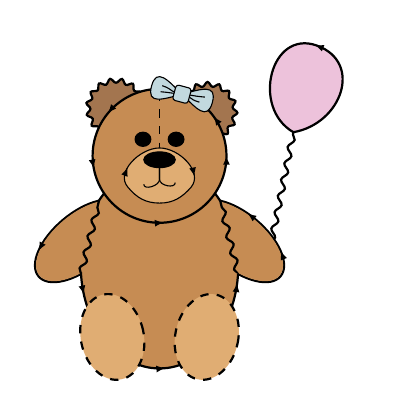
\begin{tikzpicture}[scale=1.0]
  
  \def\bw{1.00} % body
  \def\bh{1.30}
  \def\aa{130}  % arms
  \def\aw{0.35}
  \def\ah{0.70}
  \def\fa{12}   % feet
  \def\fw{0.4}
  \def\fh{0.55}
  \def\ea{130}  % ears
  \def\ew{0.35}
  \def\eh{0.35}
  \def\hw{0.85} % head
  \def\hh{0.85}
  \def\nw{0.40} % nose
  \def\nh{0.70}
  
  \coordinate (B)  at ( 1.0,  1.2  );
  \coordinate (LA) at ( 0.0,  1.52 );
  \coordinate (RA) at ( 2.0,  1.52 );
  \coordinate (LF) at ( 0.4,  0.3  );
  \coordinate (RF) at ( 1.6,  0.3  );
  \coordinate (H)  at ( 1.0,  2.6  );
  %\coordinate (LE) at ( 0.4,  3.1 );  % ear
  %\coordinate (RE) at ( 1.6,  3.1 );
  \path (H) +(135:0.97*\hh) coordinate (LE);
  \path (H) +( 45:0.97*\hh) coordinate (RE);
  \path (H) +( 70:0.98*\hh) coordinate (X); % bow
  \path (H) +(135:0.35*\hh) coordinate (LY);
  \path (H) +( 45:0.35*\hh) coordinate (RY);
  \coordinate (T)  at ( 1.0,2.6+0.8);
  \coordinate (N)  at ( 1.0,2.6+0.1);
  %\coordinate (LY) at ( 0.8,2.6+0.2); % eye
  %\coordinate (RY) at ( 1.2,2.6+0.2);
  
  % BALLOON
  \draw[thick,decorate,decoration={snake,segment length=6,amplitude=1}]
      (2.4,1.4) --++(+0.3,1.5);
  \draw[thick,fill=myred]
      (2.4,1.4) ++(+0.3,1.5) to[out=10,in=-20,looseness=1.4] ++(+0.3,+1.1)
                             to[out=-200,in=150,looseness=1.4] ++(-0.3,-1.1);
  
  % ARMS & BODY & LEGS
  \draw[thick,rotate= \aa,name path=LA]
    (LA) ellipse ({\aw} and {\ah});
  \draw[thick,rotate=-\aa,name path=RA]
    (RA) ellipse ({\aw} and {\ah});
  \draw[thick,fill=mybrown,name path=B]
    (B)  ellipse ({\bw} and {\bh});
  \draw[thick,dashed,fill=lightbrown,rotate= \fa]
    (LF) ellipse ({\fw} and {\fh});
  \draw[thick,dashed,fill=lightbrown,rotate=-\fa]
    (RF) ellipse ({\fw} and {\fh});
  
  % ARMS WITH BOSON LINES
  \begin{scope}
    \path[name intersections={of=B and LA, name=i}];
    \clip[rotate=\aa] (LA) ellipse ({\aw} and {\ah});
    \fill[mybrown,rotate=\aa] (LA) ellipse ({0.97*\aw} and {0.98*\ah});
    \draw[thick,fill=mybrown,decorate,decoration={snake,segment length=6,amplitude=1}]
      (i-2) -- (i-1);
  \end{scope}
  \begin{scope}
    \path[name intersections={of=B and RA, name=i}];
    \clip[rotate=-\aa] (RA) ellipse ({\aw} and {\ah});
    \fill[mybrown,rotate=-\aa] (RA) ellipse ({0.97*\aw} and {0.98*\ah});
    \draw[thick,fill=mybrown,decorate,decoration={snake,segment length=6,amplitude=1}]
      (i-2) -- (i-1);
  \end{scope}
  
  % EARS & HEAD
  \draw[thick,fill=darkbrown,rotate={180+\ea},
        decorate,decoration={snake,segment length=4,amplitude=0.8}]
    (LE) ellipse ({\ew} and {\eh});
  \draw[thick,fill=darkbrown,rotate=-\ea,
        decorate,decoration={snake,segment length=4,amplitude=0.8}]
    (RE) ellipse ({\ew} and {\eh});
  \draw[thick,fill=mybrown]
    (H)  ellipse ({\hw} and {\hh});
  
  % NOSE & EYES & MOUTH
  \draw[dashed] (T) --++ (0,-0.8);
  \draw[fill=lightbrown,
        postaction={decorate},arrowmarka={0.25}{7},arrowmarka={0.80}{10}]
    (N) to[out=0,in=50] ++(\nw,-0.5) to[out=-132,in=0] ++(-\nw,-0.2)
    to[out=180,in=-50] ++(-\nw,0.2) to[out=132,in=180] (N);
  \draw[fill=black] (N)++(0,-0.15) ellipse (0.2 and 0.1);
  \draw[fill=black] (LY) ellipse (0.10 and 0.09);
  \draw[fill=black] (RY) ellipse (0.10 and 0.09);
  %\fill[white] (LY) ++(88:0.035) ellipse (0.02 and 0.01);
  %\fill[white] (RY) ++(88:0.035) ellipse (0.02 and 0.01);
  \draw
    (N)++(0,-0.1) --++ (0,-0.3) to[out=-90,in=-90] ++(-0.2,-0.06);
  \draw
    (N)++(0,-0.1) --++ (0,-0.3) to[out=-90,in=-90] ++(+0.2,-0.04);
  
  % ARROWS
  \path[postaction={decorate},
    %arrowmark={0.20},arrowmark={0.33},
    arrowmark={0.55},arrowmark={0.76},arrowmark={0.97}]
    (B)  ellipse ({\bw} and {\bh});
  \path[rotate= \aa,postaction={decorate},arrowmarka={0.15}{-5}]
    (LA) ellipse ({\aw} and {\ah});
  \path[rotate=-\aa,postaction={decorate},arrowmarka={0.35}{-2},arrowmarka={0.54}{-2}]
    (RA) ellipse ({\aw} and {\ah});
  \path[postaction={decorate},
        arrowmark={0.0},arrowmark={0.10},arrowmark={0.39},arrowmark={0.53},arrowmark={0.76}]
    (H)  ellipse ({\hw} and {\hh});
  \path[postaction={decorate},arrowmarka={0.50}{-5}]
      (2.4,1.4) ++(+0.3,1.5) to[out=  10,in=-20,looseness=1.4] ++(+0.3,+1.1)
                             to[out=-200,in=150,looseness=1.4] ++(-0.3,-1.1);
  
  % BOW
  \begin{scope}[rotate=-15]
    \draw[fill=myblue]
      (X) to[out= 30,in=  90,looseness=1.6] ++(+0.4,0)
          to[out=-90,in= -30,looseness=1.6] (X)
          to[out=150,in=  90,looseness=1.6] ++(-0.4,0)
          to[out=-90,in=-150,looseness=1.6] (X);
    \draw
      (X) to[out=10,in=-170,looseness=1.6] ++(+0.29,+0.04);
    \draw
      (X) ++(0,-0.01) to[out= 6,in= 180,looseness=1.6] ++(+0.24,-0.03);
    \draw
      (X) to[out=-170,in=10,looseness=1.6] ++(-0.27,-0.04);
    \draw
      (X) ++(0,+0.01) to[out=-170,in=-4,looseness=1.6] ++(-0.27,+0.03);
    \draw[fill=myblue,rounded corners=1]
      (X) ++(-0.1,-0.1) rectangle ++ (+0.2,+0.2);
  \end{scope}
  
\end{tikzpicture}


\end{document}